\section{Solution Technique}

Assuming the values for $C$ and $M$ at time level $k$ are known, (\ref{equ:M_space_discret}) and (\ref{equ:C_space_discret}) are a coupled system of $2nm$ highly nonlinear equation for $2nm$ unknown $M^{k+1}_{l}$, $C^{k+1}_{l}$.
To solve this coupled system, we define a fixed point iteration: 
\begin{equation}
  M^{(p)}_{l} := M^{k}_{l}, \quad C^{(p)}_{l} := C^{k}_{l},
\end{equation}
which we apply to (\ref{equ:M_space_discret}) and (\ref{equ:C_space_discret}).
In a single time step, the solutions for $M$ and $C$ can be solved using the previous time step solution in the follow manner:
\begin{equation} \label{equ:M_fixed_point}
  \frac{M^{(p+1)}_{l} - M^{k}_{l}}{\Delta t} = 
    \frac{1}{\Delta x^2} \sum_{\sigma \in \mathcal{N}_{ij}}
    \left( \frac{D(M^{(p)}_{\sigma}) + D(M^{(p)}_{l})}{2} \right)
    \cdot \left( M^{(p+1)}_{\sigma} - M^{(p+1)}_{l} \right)
    + F(C^{(p)}_{l}) M^{(p+1)}_{l}
\end{equation}
\begin{equation} \label{equ:C_fixed_point}
  \frac{C^{(p+1)}_{l} - C^{k}_{l}}{\Delta t} = \frac{1}{2} ( G(C^{(p+1)}_{l} ) M^{(p+1)}_{l} + G(C^{k}_{l}) M^{k}_{l} )
\end{equation}
where $(p) \in (0,1,2,\ldots)$
The fixed-point iteration is stopped when convergence is acheived.
This is when the difference between consecutive iterations is below a selected tolerance, i.e.
\begin{equation}
  \sum^{n}_{l} \left( \left| M^{(p+1)}_{l} - M^{(p)}_{l}\right| + \left| C^{(p+1)}_{l} - C^{(p)}_{l} \right| \right) < tol.
\end{equation}
At the end of the fixed-point iteration, the number of iterations is recorded as $P$, and we define,
\begin{equation}
  M^{k+1}_{l} := M^{(P)}_{l}, \quad C^{k+1}_{l} := C^{(P)}_{l}.
\end{equation}
In this fixed point format, given by (\ref{equ:M_fixed_point}) - (\ref{equ:C_fixed_point}), the equations can be rearranged and solved by conventional methods.

In each iteration step, (\ref{equ:M_fixed_point}) is a simultaneous linear system for the $nm$ unknown $M^{(p+1)}_{l}$.
From this a linear system of equations can be created following \cite{saad2003iterativeMethod}.
For each grid point, $l$ a linear system is defined as:

\begin{equation} \label{equ:M_linear_equation}
\begin{aligned}
  \frac{M^{k}_{l}}{\Delta t} &= 
  \sum_{\sigma \in \mathcal{N}_{ij}} \left( \frac{D(M^{(p+1)}_{\sigma}) + D(M^{(p+1)}_{l})} 
    {2\Delta x^2} \cdot M^{(p+1)}_{\sigma} \right) \\
  & +\sum_{\sigma \in \mathcal{N}_{ij}} \left( \left( \frac{ D(M^{(p+1)}_{\sigma}) + D(M^{(p+1)}_{l})} 
    {2\Delta x^2} \right) - F(C^{(p)}_{l}) + \frac{1}{\Delta t} \right) M^{(p+1)}_{l}.
\end{aligned}
\end{equation} 

From (\ref{equ:M_linear_equation}), a five-diagonal matrix can be created defined as,
%!%\begin{figure}
%  \centering
%  \begin{tikzpicture}[scale = 2]
%    \draw[thick] (0,0) -- (3,0) -- (3,3) -- (0,3) -- (0,0);
%    \draw[dashed] (0,0) grid (3,3);
%  \end{tikzpicture}
%  \caption{The pattern of matrix associated with the linear system formed by finite difference method.}
%  \label{fig:matrixPattern}
%\end{figure}
% Some time find a better way to represent this matrix. Try copying Saad maybe?
%!% Hermann: I think you need to redifne your matrix A, as your notation is very unclear. For example in the ith row of the matrix some entries are a_{i,*} other a_{i-1,*} etc similar for columns.  My gues is that without explicitly introducing your grid ordering here, you will not be able to write this matrix cleanly. So maybe this is what you should do. I also suggest to not use i,j,k,p,m,n for the columns/rows of the matrix as these "counters" are already used in a different context.
\begin{equation} \label{equ:M_matrix_form}
  A = 
    \left( 
      \begin{array}{c c c c c c c c c c}
        A_{1} & a_{2} &  & a_{m} &   \\
        a_{1} & A_2 & a_3 &   &  a_{m+1} &   \\
        & \ddots & \ddots & \ddots & & \ddots & \\
        a_{1} &  & a_{n-1} & A_{n} & a_{n+1} &   &  a_{n+m} &   \\
        & \ddots & & \ddots & \ddots & \ddots & & \ddots\\
        & & a_{(n-1)m - m} &  & a_{(n-1)m-1} & A_{(n-1)m} & a_{(n-1)m+1} &  & a_{(n-1)m +m} \\
        & & & \ddots & & \ddots & \ddots & \ddots & \\
        & & & & a_{n(m-1)-1} & & a_{nm-2} & A_{nm-1} & a_{nm} \\
        & & & & & a_{n(m-1)} & & a_{nm-1} & A_{nm}
      \end{array}
    \right)
\end{equation}
where each $A_l$ is the diagonal coefficient and $a_{l}$ is the off-diagonal coefficient based on (\ref{equ:M_linear_equation}). 

\begin{prop}
  The matrix $A$ is positive definite and symmetric when $ \Delta t < \left( { F(C^{(p)}_{l}) } \right)^{-1}$.
\end{prop}
\begin{proof}
  Matrix $A$ is positive definite if all the eigenvalues are positive. 
  Using the Circle theorem described by \cite{varga2004gersgorin}, the eigenvalues can be shown to be positive if, independently on all rows, the sum of the off-diagonals values is less then the diagonal value.
  This can be verified. From (\ref{equ:M_linear_equation}) it can be said that,
  \begin{equation} \label{equ:diagonalGreatOffdiagonal}
    \left| \sum_{\sigma \in \mathcal{N_{ij}}} \left( \frac{D( M^{(p)}_{\sigma} )}{\Delta x^2} \right) \right|
     < \left| \left( \sum_{\sigma \in \mathcal{N_{ij}}} \left( \frac{D( M^{(p)}_{\sigma} )}{\Delta x^2} \right) 
    - F(C^{(p)}_{l}) + \frac{1}{\Delta t} \right) \right|.
  \end{equation}
  This simplifies to,
  \begin{equation}
    \frac{1}{\Delta t} < F(C^{(p)}_{l})
  \end{equation}

  The symmetry of $A$ can be trivially shown if one considers the formation of the diagonals.
  On a single row, each element corresponds to the adjacent grid points of grid $l$.
  As the grid ordering counts along, the elements that are equidistance from the diagonal are actually reference to the same grid point. 
  Therefore we have symmetry. 
\end{proof} 

It is important to remark that this condition for which $A$ is positive definite and symmetric is practically not a severe constraint.
The condition, $\frac{1}{F(C)} < \Delta t$, relates the growth of the biomass to the size of timestep selected.
In order to resolve any biomass growth, $\Delta t$ must obviously be chosen smaller then the characteristic time scale of growth ,$\frac{1}{F(C)}$.

Given that $A$ is positive definite and symmetric, the conjugate gradiant method can be used to compute the solution.

\begin{prop}
  The matrix $A$ is diagonally dominate when $\Delta t < \left( { F(C^{(p)}_{l}} \right)^{-1}$.
\end{prop}
\begin{proof}
  This is trivially shown to be true when one considers (\ref{equ:diagonalGreatOffdiagonal}).
  It was shown that this simplifies to 
  \begin{equation}
    \frac{1}{\Delta t} < F(C^{(p)}_{l}).
  \end{equation}
  This means that when the above is true the diagonal elements of $A$ will be strictly larger then the sum of off-diagonals.
  Therefore we have diagonal dominance.
\end{proof}
Since we have $A$ positive definite, symmetric, and diagonally dominate we know that $A$ is an M-matrix.
This is important because this ensures that if $M^k$ is non-negative we have that $M^{(p)}$ is also non-negative.

For solving (\ref{equ:C_fixed_point}), the equation can be rearranged into a quadratic form, substituting in $G(C)$ from (\ref{equ:model_functions})
\begin{equation} \label{equ:quadratic_C}
  \left(C^{(p+1)}\right)^2 + \left( \kappa - C^k + \frac{\Delta t}{2} \gamma M^{(p+1)} + \frac{\Delta t}{2} \frac{ \gamma C^k M^k}{\kappa + C^k} \right) C^{(p+1)} + \left( -\kappa C^k + \frac{\Delta t}{2} \frac{\gamma \kappa C^k M^k}{\kappa + C^k} \right) = 0.
\end{equation}

Using the quadratic equation results in, 
  \begin{equation} \label{eq:Cquad}
    C^{(p+1)} = \frac{-b \pm \sqrt{b^2 - 4c}}{2}
  \end{equation}  
  for which, 
  \begin{equation} \begin{aligned} \label{para:abc}
    b &= \kappa - C^k + \frac{\Delta t}{2} \gamma M^{(p+1)} + \frac{\Delta t}{2} \frac{\gamma C^k M^k}{\kappa + C^k} \\
    c &= -\kappa C^k + \frac{\Delta t}{2} \frac{\gamma \kappa C^k M^k}{\kappa + C^k}
  \end{aligned}  \end{equation}

Unless $b^2 - 4c = 0$, we have two different solutions to $C^{(p+1)}$. 
The problem with that is that if both solutions are positive we have two valid values to be used. 
Here, we can show that there will always be only one positive solution.

\begin{prop}
  The quadratic equation defined as (\ref{equ:quadratic_C}) will always have one positive solution and one negative solution for non-zero parameter choices.
\end{prop}

\begin{proof}
  Rearranging (\ref{equ:quadratic_C}) so that all the $\Delta t$ terms are on the right-hand-side, we get
  \begin{equation}
    \left( C^{(p+1)} \right)^2 + \left(\kappa - C^{k}\right)C^{(p+1)} - \kappa C^{k} =  \left(\frac{\gamma C^k M^k}{2\left(\kappa + C^k\right)} - \left(\frac{\gamma M^{(p+1)}}{2} - \frac{\gamma C^k M^k}{2 \left(\kappa + C^k\right)} \right)C^{(p+1)} \right) \Delta t.
  \end{equation}
  To simplify the notation, we let $\bar{a} := \frac{\gamma M^{(p+1)}}{2} - \frac{\gamma C^k M^k}{2\left(\kappa + C^k\right)}$ and $\bar{b} := \frac{\gamma C^k M^k}{2\left(\kappa + C^k\right)}$.
  
%!% Hint:  you can simplify the notation if you drop the index (p+1) here. C^{(p+1)} is the dummy argument of both functions; you might as well call it C.
  We analysize both the left-hand-side and right-hand-side independently by letting $f_l = \left( C^{(p+1)} \right)^2 + \left(\kappa - C^{k}\right)C^{(p+1)} - \kappa C^{k}$ and $f_r =  \left(\bar{b} - \bar{a} C^{(p+1)} \right) \Delta t$.
  $f_l$ is a quadratic equation with positive concavity everywhere and $C^{(p+1)}$-intercept at $-\kappa C^{k} < 0$.
  $f_r$ is a line with a slope opposite to the sign of $\bar{a}$ and has $C^{(p+1)}$-intercept at $\bar{b}\Delta t > 0$.
  Refer to Figure (\ref{fig:proof_pos_sol}) for a visual of $f_l$ and $f_r$.
%!% l.233 ... correct me if I am wrong, but i think you have for cases:  the minimum of the quadratic function either in the left half plane or in the right half plane, the linear function either down or up.  gives four different parings. if you draw each of them then it becomes pretty clear what the situation is. Again, we can discuss and tidy up when we meet.
  
  Consider the case $\bar{a} < 0$.
  This means that $f_r$ has a positive slope.
  We can show that $f_r$ must intersect with $f_l$ twice, one at $C^{(p+1)} <0$ and another at $C^{(p+1)}$.

  For the positive intersection we can consider a point $c > 0$.
  Because $f_l = O\left((C^{(p+1)})^2 \right)$, using Big-$O$ notation, and $f_r = O\left(C^{(p+1)}\right)$ we know that there exists a $c$ for which $f_l > f_r$ for all $C^{(p+1)} > c$.
  Since we trivially have $f_r(0) > f_l(0)$ we can use the intermediate value theorem to determine that there must exist a intersection between $f_l$ and $f_r$.
  This intersection is the point where $f_l = f_r$ and satisfies our equation resulting in a solution for $C^{(p+1)} > 0$. 
  For the negative intersection we know that $f_r(0) > f_l(0)$ and $f_r$ is monotonically increasing with $C^{(p+1)}$ and $f_l$ is monotonically decreasing for $C^{(p+1)} < 0$.
  This means that there must exist a point where the two functions intersect and thus we have a solution for $C^{(p+1)} < 0$.

  The other case of $\bar{a} < 0$ follows a similar argument to the previous and also results in one positive solution and one negative solution for (\ref{equ:quadratic_C}).
  
\end{proof}


\begin{figure}
  \centering
  \begin{tabular}{c c}
  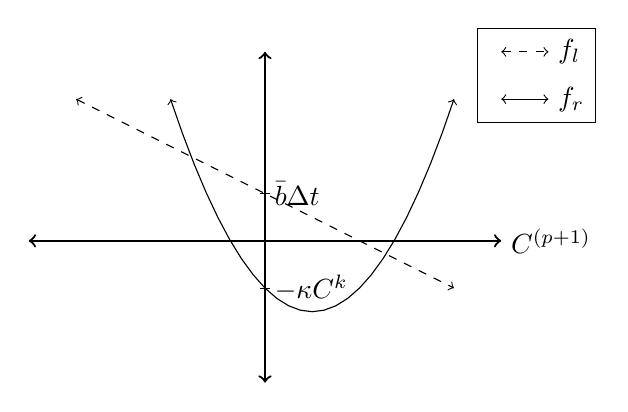
\begin{tikzpicture}[scale=0.6]
    \draw[<->, thick] (-5, 0) -- (5, 0);
    \draw[<->, thick] (0, -3) -- (0, 4); 
    \node[right] at (5, 0) {$C^{(p+1)}$};
    \node[above] at (0, 4) {};

    \draw[<->, domain=-2:4] plot (\x, {0.5*\x*\x - \x - 1});
    \draw (-0.1, -1) -- (0.1, -1);
    \node[right] at (0, -1) {$-\kappa C^{k}$};

    \draw[<->, dashed, domain=-4:4] plot (\x, {-0.5*\x+1});
    \draw (-0.1, 1) -- (0.1, 1); 
    \node[right] at (0, 1) {$\bar{b} \Delta t$};

    \draw (7, 2.5) -- (4.5, 2.5) -- (4.5, 4.5) -- (7, 4.5) -- (7, 2.5);
    \draw[<->, dashed] (5, 4) -- (6, 4);
    \node[right] at (6, 4) {$f_l$};
    \draw[<->] (5, 3) -- (6, 3);
    \node[right] at (6, 3) {$f_r$};

  %!%  \node[left] at (-4,-3) {$\bar{a} > 0, \kappa - C^k  < 0$};
  \end{tikzpicture}
  &
  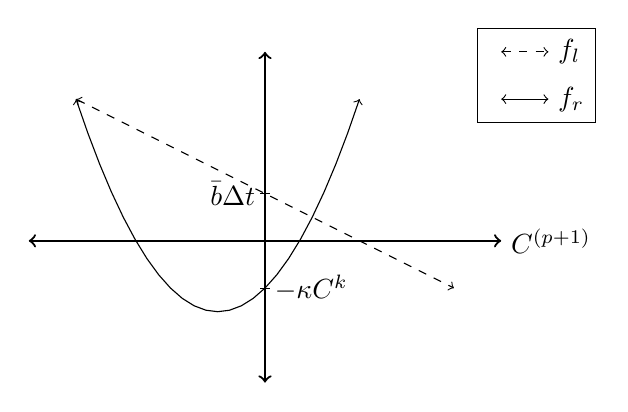
\begin{tikzpicture}[scale=0.6]
    \draw[<->, thick] (-5, 0) -- (5, 0);
    \draw[<->, thick] (0, -3) -- (0, 4); 
    \node[right] at (5, 0) {$C^{(p+1)}$};
    \node[above] at (0, 4) {};

    \draw[<->, domain=-4:2] plot (\x, {0.5*\x*\x + \x - 1});
    \draw (-0.1, -1) -- (0.1, -1);
    \node[right] at (0, -1) {$-\kappa C^{k}$};

    \draw[<->, dashed, domain=-4:4] plot (\x, {-0.5*\x+1});
    \draw (-0.1, 1) -- (0.1, 1); 
    \node[left] at (0, 1) {$\bar{b} \Delta t$};

    \draw (7, 2.5) -- (4.5, 2.5) -- (4.5, 4.5) -- (7, 4.5) -- (7, 2.5);
    \draw[<->, dashed] (5, 4) -- (6, 4);
    \node[right] at (6, 4) {$f_l$};
    \draw[<->] (5, 3) -- (6, 3);
    \node[right] at (6, 3) {$f_r$};
  \end{tikzpicture}
  \\
  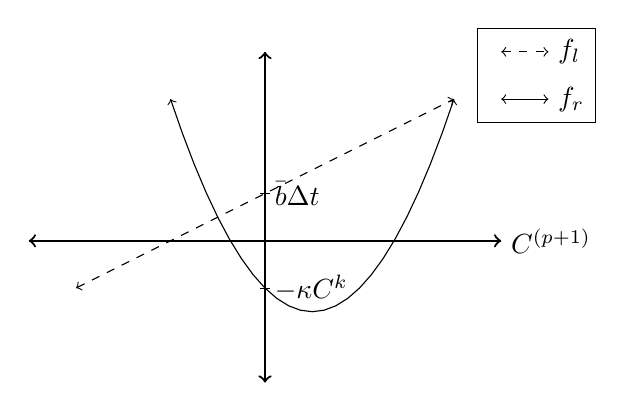
\begin{tikzpicture}[scale=0.6]
    \draw[<->, thick] (-5, 0) -- (5, 0);
    \draw[<->, thick] (0, -3) -- (0, 4); 
    \node[right] at (5, 0) {$C^{(p+1)}$};
    \node[above] at (0, 4) {};

    \draw[<->, domain=-2:4] plot (\x, {0.5*\x*\x - \x - 1});
    \draw (-0.1, -1) -- (0.1, -1);
    \node[right] at (0, -1) {$-\kappa C^{k}$};

    \draw[<->, dashed, domain=-4:4] plot (\x, {0.5*\x+1});
    \draw (-0.1, 1) -- (0.1, 1); 
    \node[right] at (0, 1) {$\bar{b} \Delta t$};

    \draw (7, 2.5) -- (4.5, 2.5) -- (4.5, 4.5) -- (7, 4.5) -- (7, 2.5);
    \draw[<->, dashed] (5, 4) -- (6, 4);
    \node[right] at (6, 4) {$f_l$};
    \draw[<->] (5, 3) -- (6, 3);
    \node[right] at (6, 3) {$f_r$};
  \end{tikzpicture}
  & 
  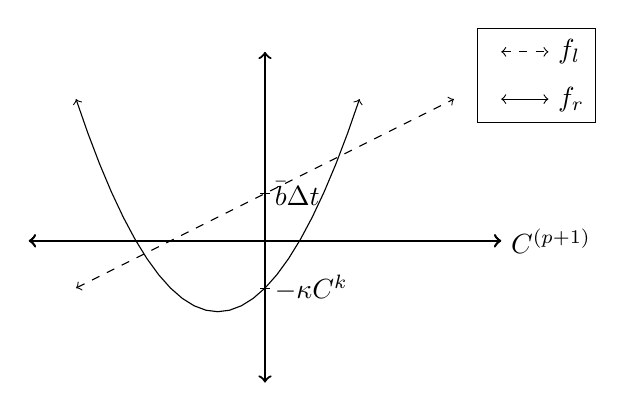
\begin{tikzpicture}[scale=0.6]
    \draw[<->, thick] (-5, 0) -- (5, 0);
    \draw[<->, thick] (-5, 0) -- (5, 0);
    \draw[<->, thick] (0, -3) -- (0, 4); 
    \node[right] at (5, 0) {$C^{(p+1)}$};
    \node[above] at (0, 4) {};

    \draw[<->, domain=-4:2] plot (\x, {0.5*\x*\x + \x - 1});
    \draw (-0.1, -1) -- (0.1, -1);
    \node[right] at (0, -1) {$-\kappa C^{k}$};

    \draw[<->, dashed, domain=-4:4] plot (\x, {0.5*\x+1});
    \draw (-0.1, 1) -- (0.1, 1); 
    \node[right] at (0, 1) {$\bar{b} \Delta t$};

    \draw (7, 2.5) -- (4.5, 2.5) -- (4.5, 4.5) -- (7, 4.5) -- (7, 2.5);
    \draw[<->, dashed] (5, 4) -- (6, 4);
    \node[right] at (6, 4) {$f_l$};
    \draw[<->] (5, 3) -- (6, 3);
    \node[right] at (6, 3) {$f_r$};
  \end{tikzpicture}
\end{tabular}
\caption{Graph of $f_l = \left( C^{(p+1)} \right)^2 + \left(\kappa - C^{k}\right)C^{(p+1)} - \kappa C^{k}$ and $f_r =  \left(\bar{b} - \bar{a} C^{(p+1)} \right) \Delta t$ for all four possible cases.
  Notice that because $-\kappa C^{k} < 0$ and $\bar{b} \Delta t > 0$ for all realistic parameter values the two functions will always intersect in the positive $C^{(p+1)}$ region.
  The top left graph is for $\bar{a} > 0$ and $\kappa - C^k < 0$.
  The top right graph is for $\bar{a} > 0$ and $\kappa - C^k > 0$.
  The bottom left graph is for $\bar{a} < 0$ and $\kappa - C^k < 0$.
  The bottom right graph is for $\bar{a} < 0$ and $\kappa - C^k > 0$.
}
\label{fig:proof_pos_sol}
\end{figure}
  
%!% l.247-l.259  is this needed?  didn't you already answer/explain this with Prop. 3.2.2
To determine which branch of (\ref{eq:Cquad}) to use, a physical situation is used. 
Specifically the case where there exist no biomass, $M = 0$. 

The expected outcome is that no substrate is consumed and thus the substrate concentration will remain constant as a function of $t$. 
When the equations in (\ref{para:abc}) are evaluated at $M = 0$, the result it,
\begin{equation}
  b = \kappa - C^k, \quad c = -\kappa C^k,
\end{equation} 
which can be used to evaluate (\ref{eq:Cquad}) as,
\begin{equation} \begin{aligned}
  C^{(p+1)} &= \frac{- (\kappa - C^k) \pm \sqrt{(\kappa - C^k)^2 - 4 (-\kappa C^k)}}{2} \\
    &= \frac{1}{2} \left( C^k - \kappa \pm \sqrt{\kappa^2 + 2 \kappa C^k + \left(C^k \right) ^2}\right) \\
    &= \frac{1}{2} \left( C^k - \kappa \pm (\kappa+C^k) \right). \\
\end{aligned} \end{equation}
Now, if the positive branch is used the above equation evaluates to $C^{(p+1)} = C^k$. 
This means that between any two distinct times, the substrate concentration will remain constants, which was expected. 
To further this confirmation, the negative branch results in $C^{(p+1)} = -\kappa $, a non-postive substrate concentration, which is not physically relavent. 
\begin{equation}
  C^{(p+1)} = \frac{-b + \sqrt{b^2 - 4c}}{2}
\end{equation} 
where $b$ and $c$ are defined in (\ref{para:abc}).
%!% Maybe instead we can just get a trivial explaination from the fact that sqrt() is always positive so the only positive C is going be from the positive branch

Now that computable solutions for $M$ and $C$ at a single time step have been found, an algorithm to solve for the next time step can be established.
Algorithm \ref{alg:iterateCM} shows the organization of solving (\ref{equ:C_fixed_point} - \ref{equ:M_fixed_point}). 
\begin{algorithm}
  \KwData{$M^{k}$, $C^{k}$ are vectors with values from the previous timestep and $p = 0$. }
  \Begin
  {
    Let $M^{(0)} = M^{k}$ and $C^{(0)} = C^{k}$\;
    \While{Convergence is not acheived } 
    {
        Solve $A^{(p)} M^{(p+1)} = b^{(p)}$\;
        Solve $C^{(p+1)} = \frac{1}{2} \left( b \pm \sqrt{b^2 - 4c} \right)$\;
        Check convergence\; 
        Let $C^{(p)} = C_{(p+1)}$\;
        Let $M^{(p)} = M_{(p+1)}$\;
        Let $p = p + 1 $\;
    }
    Let $M^{(k+1)} = M^{(P)}$ and $C^{(k+1)} = C^{(P)}$\;
  }
  \caption{Algorithm for the fully-implicit solving of (\ref{equ:model_system}) }
  \label{alg:iterateCM}
\end{algorithm}

Note that Algorithm \ref{alg:iterateCM} actually describes both a fully- and semi- implicit method for solving (\ref{equ:model_system}). 
If $P = 1$ then only a single iteration of the algorithm is applied, which correlates to a semi-implicit method would behave.
This can be produced by selecting a sufficiently large enough tolerance so that the convergence check is always resolved after the first iteration.
The resulting semi-implicit method is effectivly the same as one described in \cite{sirca2012computational}.



